\documentclass[11pt, a4paper]{article}
\usepackage[utf8]{inputenc}
\usepackage{t1enc}
\usepackage[magyar]{babel}
\usepackage{lmodern}
\usepackage{url}
\usepackage{graphics}
\usepackage{listings}
\usepackage[a4paper, total={5.3in, 8in}]{geometry}

\sloppy

\begin{document}
\title{Szoftver architektúrák \\ Szótanulást segítő alkalmazás \\ \large{Rendszerterv}}
    \author{Graics Bence \and Verbőczy Kristóf}

    \maketitle
    
    \tableofcontents
    \newpage
    
    \section{Bevezetés}
    \label{sec:bevezetes}
    Jelen dokumentum a Szoftver architektúrák nevű tárgyra kidolgozott házi feladat rendszertervet mutatja be. A házi feladat során a cél egy szótanulást segítő alkalmazás megtervezése és implementálása volt. A követelmények és a specifikáció a ... érhető el.
    
    A dokumentum a következők szerint épül fel:
    
    \section{Architektúra}
    \label{sec:architektúra}
    Jelen fejezet bemutatja az elkészített szótanuló alkalmazás architektúráját, azaz hogy \textit{1)} a rendszer milyen komponensekből épül fel, \textit{2)} az egyes komponenseknek milyen lényeges elemei vannak, \textit{3)} a komponensek hogyan kapcsolódnak egymáshoz.
    
    Az általunk tervezett rendszer egy adatközpontú alkalmazás, amely kliens-szerver architektúrát követ. A szerver tárolja a szükséges adatokat, például a felhasználók adatait és az egyes leckékhez tartozó adatokat (szavakat és képeket). A kliens feladata, hogy a felhasználó kérésére fogyasztható formában tárja a felhasználó elé ezen adatokat, és kezelje az esetleges interakciókat. Az adatok (az objektum-orientáltság szabályai szerint) objektumokban (DTO) kerülnek továbbításra és feldolgozásra. A szerver és a kliens kommunikációját jól meghatározott interfészek teszik lehetővé.
    
    \subsection{Objektumok}
    
    \subsection{Interfészek}
    
    \subsection{A szerver}
    
    \subsection{A kliens}
    \label{sec:kliens}
    A kliens a következő feladatokat látja el, felhasználva a szerver által nyújtott szolgáltatásokat.
    \begin{enumerate}
    	\item Megjelenít különböző adatokat. Ezen adatok tartozhatnak egy adott felhasználóhoz, pl.~név, pontszám, tudásszint, vagy tartozhat leckékhez, pl. angol szó, magyar szó, objektumot leíró kép.
    	\item Felhasználói kéréseket hajt végre az alkalmazáslogikának megfelelően. Ezek közé tartozik egy lecke megtanítása (tanítási folyamat végrehajtása), leckék kilistázása, leckék felvétele és törlése, felhasználók létrehozása és törlése (adminisztrátor felhasználó esetén).
    	\item A felhasználói kérések teljesítéséhez felveszi a kapcsolatot a szerverrel, hogy lekérje a szükséges adatokat, illetve perzisztálja adatok módosításának az eredményét.
    \end{enumerate}

	A kliens egy réteges felépítést követ, minden réteghez egy fent meghatározott feladat társul. A kliens felépítését \aref{fig:client-arch}.~ábra mutatja be.
	       \begin{figure}[htbp]
	       	\center
	       	\resizebox{60mm}{!}{
	       		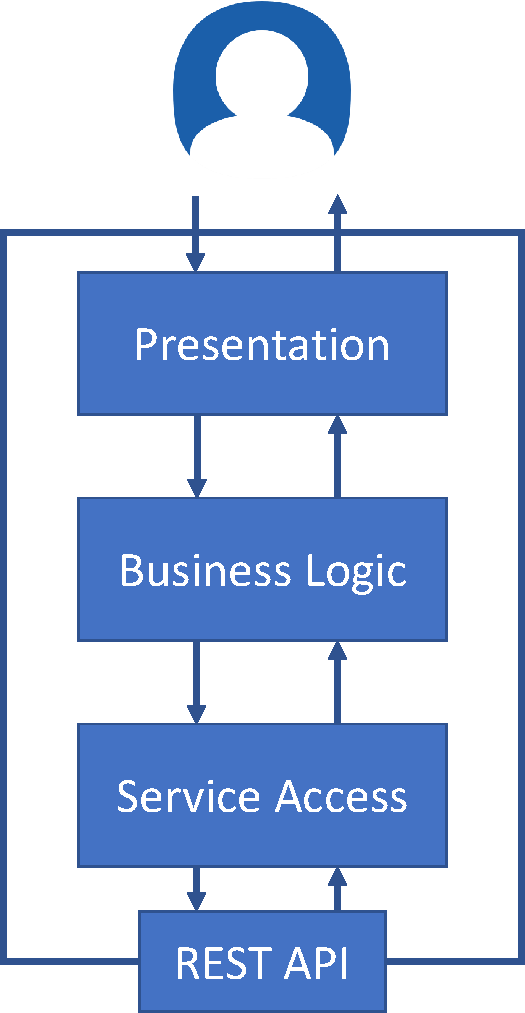
\includegraphics{figures/client-arch.pdf}
	       	}
	       	\caption{A kliens architektúrája.}
	       	\label{fig:client-arch}
	       \end{figure}
	
	Amint látható, a kliens egy tisztán rétegelt architektúrát valósít meg. A megjelenítési réteg csak az üzleti logikai réteg  nyújtotta szolgáltatásokat használja fel, az üzleti logikai réteg pedig csak a szolgáltatás hozzáférési rétegre támaszkodik. Az alkalmazásban egy réteget egy osztály valósít meg. A következő szekciók részletesebben bemutatják az egyes rétegek megvalósítását.
     
     \subsubsection{Megjelenítési réteg: View osztály}
     A View osztály felelős a grafikus felhasználói felület megvalósításáért. A grafikus felület a JavaFX FXML technológia felhasználásával került definiálásra. Ennek segítségével a felületen található vezérlőket deklaratív jelleggel lehet definiálni az XML szintaktikának megfelelően: vezérlő hierarchiákat lehet létrehozni, illetve az egyes vezérlők tulajdonságait lehet definiálni (méret, szín, elrendezési algoritmus). A következő kódrészlet a bejelentkezéshez szükséges vezérlők definiálását mutatja be.
     
\begin{lstlisting}
tartalom...
\end{lstlisting}
     
     A grafikus felület egy \emph{egyablakos} megközelítést követ; az egyes funkciók különböző \emph{tabokon} keresztül érhetők el. A következőkben bemutatjuk a legfontosabb képernyőket, amelyek az alkalmazás jelentősebb funkcionalitásaihoz tartoznak.
     
     A program indulása utána a következő képernyő fogad (lásd \ref{} ábra).     
     %       \begin{figure}[htbp]
     %       	\center
     %       	\resizebox{140mm}{!}{
     %       		\includegraphics{messageformat.pdf}
     %       	}
     %       	\caption{Chat üzenet formátum}
     %       	\label{fig:messageformat}
     %       \end{figure}
     A felhasználónak lehetősége van bejelentkezni. Rossz felhasználónév vagy jelszó esetén az alkalmazás egy felugró ablakkal figyelmeztet (\ref{} ábra).
     %       \begin{figure}[htbp]
     %       	\center
     %       	\resizebox{140mm}{!}{
     %       		\includegraphics{messageformat.pdf}
     %       	}
     %       	\caption{Chat üzenet formátum}
     %       	\label{fig:messageformat}
     %       \end{figure}
     Bejelentkezés után a felhasználó megvizsgálhatja jelenlegi pontjait, tudás szintjét, illetve ki is jelentkezhet.     
     %       \begin{figure}[htbp]
     %       	\center
     %       	\resizebox{140mm}{!}{
     %       		\includegraphics{messageformat.pdf}
     %       	}
     %       	\caption{Chat üzenet formátum}
     %       	\label{fig:messageformat}
     %       \end{figure}
     A tanulást, azaz egy lecke megkezdését a \emph{Start Learning!} gombra kattintva kezdheti el, ahol a három különböző feladattípushoz a következő képernyők tartoznak (\ref{}, \ref{} és \ref{} ábra).
     %       \begin{figure}[htbp]
     %       	\center
     %       	\resizebox{140mm}{!}{
     %       		\includegraphics{messageformat.pdf}
     %       	}
     %       	\caption{Chat üzenet formátum}
     %       	\label{fig:messageformat}
     %       \end{figure}
     %       \begin{figure}[htbp]
     %       	\center
     %       	\resizebox{140mm}{!}{
     %       		\includegraphics{messageformat.pdf}
     %       	}
     %       	\caption{Chat üzenet formátum}
     %       	\label{fig:messageformat}
     %       \end{figure}
     %       \begin{figure}[htbp]
     %       	\center
     %       	\resizebox{140mm}{!}{
     %       		\includegraphics{messageformat.pdf}
     %       	}
     %       	\caption{Chat üzenet formátum}
     %       	\label{fig:messageformat}
     %       \end{figure}
     Leckék kezelését (hozzáadás, törlés, listázás) a felhasználó a következő ablakon végezheti (\ref{} ábra).
     %       \begin{figure}[htbp]
     %       	\center
     %       	\resizebox{140mm}{!}{
     %       		\includegraphics{messageformat.pdf}
     %       	}
     %       	\caption{Chat üzenet formátum}
     %       	\label{fig:messageformat}
     %       \end{figure}
     Végül a grafikus felületen található egy adminisztrációs felület is, amelyet adminisztrátor felhasználók vehetnek igénybe (\ref{} ábra). Itt lehet felhasználókat törölni, illetve új felhasználókat hozzáadni az alkalmazáshoz.
     %       \begin{figure}[htbp]
     %       	\center
     %       	\resizebox{140mm}{!}{
     %       		\includegraphics{messageformat.pdf}
     %       	}
     %       	\caption{Chat üzenet formátum}
     %       	\label{fig:messageformat}
     %       \end{figure}
   
     \subsubsection{Controller}
     A Controller felelős a felhasználói interakciók kezeléséért és az alkalmazáslogika megvalósításáért. A felhasználói interakciók lekezelése handler metódusokkal történik.
     
     Az alkalamzáslogika legbonyolultabb része a leckék levezénylésének a folyamata.
     \subsubsection{Service access}
     
    \section{Telepítési útmutató}
    
%       \begin{figure}[htbp]
%       	\center
%       	\resizebox{140mm}{!}{
%       		\includegraphics{messageformat.pdf}
%       	}
%       	\caption{Chat üzenet formátum}
%       	\label{fig:messageformat}
%       \end{figure}
    

\end{document}